\documentclass[conference]{IEEEtran}
\IEEEoverridecommandlockouts

\usepackage{cite}
\usepackage{amsmath,amssymb}
\usepackage{graphicx}
\usepackage{booktabs}
\usepackage{url}
\usepackage[hidelinks]{hyperref}

\graphicspath{{figures/}{../figures/}}

\begin{document}

\title{Detection Limits of Low-Pass Cell-Free DNA Sequencing
for Haematological Cytogenetics: A Simulation Study}

\author{\IEEEauthorblockN{Shubhodeep}
\IEEEauthorblockA{\textit{Independent Researcher}\\
\url{https://github.com/shubhodeepcx/low-pass-cfDNA}}}

\maketitle

\begin{abstract}
Low-pass whole-genome sequencing of cell-free DNA is an attractive route to
reading a haematological karyotype from a blood draw, but its published
detection limits are derived almost entirely from prenatal whole-chromosome
trisomies rather than from the arm-level and sub-arm lesions that define
myeloid disease. We report an open simulation study that measures the
detectability surface of a bin-count copy-number caller across sequencing
depth, tumour fraction and lesion size, with the genome-wide false positive
rate held at five percent by calibration against held-out normal libraries. We
find three things. First, sensitivity plateaus at roughly 0.5$\times$ coverage:
increasing depth from 0.5$\times$ to 5$\times$, a tenfold increase in cost,
improves the detection limit by a median of 4.9 percent, because library-to-library
bias rather than counting noise sets the floor. Second, the detection limit
scales with the inverse square root of lesion size, so a 5.5\,Mb deletion
requires a 39.5 percent tumour fraction at 0.1$\times$ while a 434\,Mb complex
karyotype requires 7.2 percent. Third, balanced rearrangements are called at
exactly the false positive rate at every depth and tumour fraction tested, and
we give a closed form showing that the expected number of junction-spanning
molecules is $c f / 2$, independent of both genome length and fragment length.
At 0.1$\times$ and ten percent tumour fraction this is 0.004 reads, placing
junction detection three orders of magnitude beyond an untargeted low-pass run
and within reach of a 1.5\,Mb capture panel. We conclude that the copy-neutral
blind spot is a coverage-allocation problem rather than an algorithmic one. All
code, data and figures are released under an MIT licence.
\end{abstract}

\begin{IEEEkeywords}
cell-free DNA, cytogenetics, copy number variation, haematological malignancy,
low-pass sequencing, detection limits, simulation
\end{IEEEkeywords}

\section{Introduction}

Cytogenetic characterisation drives risk stratification and treatment choice in
myeloid malignancy \cite{dohner2022eln, bernard2022ipssm}. It also requires a
bone marrow aspirate, an invasive procedure that cannot be repeated often
enough to track a clone through treatment. Cell-free DNA offers a blood-based
alternative, and shallow whole-genome sequencing of plasma DNA is already
routine in prenatal aneuploidy screening \cite{lo2010maternal,
straver2014wisecondor}, where tools such as WisecondorX
\cite{raman2019wisecondorx} and ichorCNA \cite{adalsteinsson2017ichorcna} call
large copy-number changes from coverage as low as 0.1$\times$.

Two gaps separate that success from a usable haematological assay.

The first is quantitative. Published detection limits for low-pass cell-free
DNA are overwhelmingly derived for whole-chromosome trisomies in a prenatal
setting, where the abnormal fraction is often high and the lesion spans an
entire chromosome. The lesions that matter in marrow disease span two orders of
magnitude in size, from a 5\,Mb del(20q) to a complex karyotype covering more
than 400\,Mb, and no open sensitivity map exists across the joint space of
lesion size, tumour fraction and sequencing depth with specificity held fixed.
Sensitivity reported at uncalibrated specificity is not a measurement, and with
thousands of candidate segments tested per library the difference is not
subtle.

The second gap is structural, and it is the more important of the two. A
balanced translocation changes no bin's copy number. The rearrangements that
define acute promyelocytic leukaemia, chronic myeloid leukaemia, core-binding
factor leukaemia and their relatives \cite{greenberg2017mitelman} are therefore
invisible to every bin-count method, not as a matter of tuning but as a matter
of what the data contains. The literature addresses this mostly by noting it
and moving on. We think the useful response is to price the alternative.

This paper makes three contributions:

\begin{enumerate}
\item An open, reproducible detectability surface for myeloid-relevant lesions,
      spanning six depths, nine tumour fractions and ten lesions at 200
      replicate libraries per condition, with the achieved genome-wide false
      positive rate reported at every depth rather than assumed.
\item The observation and explanation of a sensitivity plateau: beyond roughly
      0.5$\times$, additional coverage is close to wasted, because the limiting
      noise source stops being Poisson and starts being library-to-library
      bias.
\item A closed-form treatment of junction-level evidence for copy-neutral
      rearrangements, showing that the required coverage scales as the inverse
      of tumour fraction and that untargeted low-pass sequencing is three
      orders of magnitude short, while a small capture panel is not.
\end{enumerate}

We deliberately do not propose a better copy-number caller. WisecondorX and
ichorCNA have had years of refinement on within-sample normalisation, GC and
mappability correction and reference-panel construction. A new entrant competes
against the incumbent's strongest axis. Measuring the class, and identifying
precisely where it cannot go, is the more useful contribution.

\section{Related Work}

\subsection{Bin-count copy-number detection}

WISECONDOR \cite{straver2014wisecondor} introduced the within-sample
normalisation scheme that defines the class: bins are compared against a
reference set of behaviourally similar bins, which removes much of the
systematic coverage bias without requiring an explicit bias model.
WisecondorX \cite{raman2019wisecondorx} extended it with improved
normalisation and segmentation and is widely treated as the reference
implementation for shallow whole-genome copy-number calling. ichorCNA
\cite{adalsteinsson2017ichorcna} approaches the same data with a hidden Markov
model that jointly estimates tumour fraction and copy-number state, which makes
it the standard choice when the tumour fraction itself is the quantity of
interest.

All of these share a dependency on read depth per bin as the sole signal, and
all share the resulting blind spot for copy-neutral events. They also share a
dependency on a reference panel of normal libraries prepared on the same
protocol, a requirement that is easy to state and expensive to satisfy.

\subsection{Coverage bias}

GC bias in high-throughput sequencing is well characterised
\cite{benjamini2012gcbias} and is the dominant systematic effect that
bin-count callers must remove. What matters for detection limits, and what is
less often modelled explicitly, is the decomposition of bias into a component
that is reproducible across libraries, which a reference panel removes, and a
component that is redrawn per library, which it cannot. Our simulation makes
that split explicit, and it is the mechanism behind the plateau we report.

\subsection{Beyond depth}

Where depth is insufficient, the field has moved to other signals. Targeted
error-suppressed sequencing of known variants achieves sensitivity far below
what untargeted sequencing allows \cite{newman2016capp}, and personalised
assays built around a patient's own rearrangements have been used to track
disease at very low tumour fractions \cite{abbosh2017phylogenetic}.
Fragmentomics exploits the non-random fragmentation of cell-free DNA
\cite{snyder2016cellfree, cristiano2019fragmentation} to detect the presence of
disease without localising a specific lesion. Our junction calculation
quantifies exactly why the targeted route is the one that works for balanced
rearrangements.

\section{Methods}

The full implementation is available \cite{lpcfdna2026}. This section states the
model precisely enough to reimplement.

\subsection{Binned genome}

The 22 autosomes are divided into fixed 500\,kb bins, giving 5{,}738 bins.
Each bin carries a GC content, a mappability and a systematic bias multiplier.
GC content is modelled as superposed sinusoids representing isochore structure
plus local variation, centred on 0.41. Mappability is drawn from a
Beta(18, 1.6) distribution attenuated towards each centromere, and bins below
0.55 are excluded, standing in for the unalignable regions every real pipeline
drops. The systematic bias multiplier is log-normal with standard deviation
0.14 and is identical in every library simulated on the same genome.

These covariates are modelled rather than read from a reference assembly, which
keeps the study free of large data dependencies. A production pipeline
substitutes measured per-bin values at two attribute assignments and nothing
downstream changes.

\subsection{Coverage model}

For bin $i$ in a library at depth $d$, the expected read count is

\begin{equation}
\mathbb{E}[y_i] = \frac{d \, b}{\ell} \cdot s_i \cdot u_i \cdot g(x_i;\kappa)
\cdot m_i \cdot r_i
\label{eq:coverage}
\end{equation}

with $b$ the bin size, $\ell$ the read length, $s_i$ the shared systematic
bias, $u_i$ a per-library bias, $g(\cdot)$ a GC efficiency curve with
per-library sharpness $\kappa$, $m_i$ mappability and $r_i$ the copy-number
ratio. Observed counts are Poisson about this expectation.

The decomposition in \eqref{eq:coverage} is the only modelling choice that
materially affects our conclusions. The term $s_i$ is identical across
libraries and is removed by reference-panel normalisation. The term $u_i$ is
log-normal with standard deviation $0.045$ and is \emph{redrawn for every
library}, so no panel can learn it. A simulation omitting $u_i$ reports
detection limits that improve without bound as coverage grows, which is both
flattering and contrary to observed behaviour.

The copy-number ratio for a clone of copy number $c_i$ present at tumour
fraction $f$ is

\begin{equation}
r_i = \frac{f c_i + (1-f) \cdot 2}{2}.
\label{eq:mixture}
\end{equation}

A single-copy loss therefore depresses expected depth by $f/2$ rather than by
$f$. This factor of two is verified directly in the test suite against a
diploid baseline on the same chromosome, which isolates the mixture arithmetic
from chromosome-specific bias.

\subsection{Lesions}

Eight copy-number lesions spanning 5.5\,Mb to 434\,Mb were simulated: del(20q)
at two sizes, del(13q), del(7q), del(5q), trisomy 8, monosomy 7, and a complex
karyotype combining five simultaneous changes. Four balanced rearrangements,
t(9;22), t(15;17), t(8;21) and inv(16), carry no copy-number change and serve
as the negative control.

\subsection{Detector}

We reimplement the approach shared by WisecondorX and ichorCNA rather than
either tool. A library is normalised to its own total, GC-corrected by a
binned-median curve over 24 GC quantile groups, and converted to per-bin
$z$ scores against a panel of 100 normal libraries. Medians rather than means
are used for the GC curve so that a true lesion cannot drag the correction
towards itself.

Candidate segments are every chromosome arm plus sliding windows of 8, 16, 32,
64, 128 and 256 bins at half-window steps, approximately 2{,}500 segments. For
each, the statistic is the Stouffer combination \cite{stouffer1949american} of
its bin $z$ scores,

\begin{equation}
T_S = \frac{1}{\sqrt{|S|}} \sum_{i \in S} z_i ,
\label{eq:stouffer}
\end{equation}

computed by prefix sums so that cost is independent of segment overlap. A
library is called abnormal if any $|T_S|$ exceeds the threshold. This is a
simpler segmentation than circular binary segmentation
\cite{olshen2004cbs} and is deliberate: a fixed segment family makes the
multiple-testing correction exact rather than approximate.

\subsection{Threshold calibration}

With roughly 2{,}500 segments tested per library, a per-segment threshold would
call something in nearly every normal library. We instead calibrate on the
distribution of the \emph{maximum} statistic. Let $M^{(j)} = \max_S |T_S^{(j)}|$
for held-out normal library $j$. The threshold at genome-wide false positive
rate $\alpha$ is the $(1-\alpha)$ quantile of $\{M^{(j)}\}$.

Three library sets are kept disjoint: 100 for the panel, 1{,}000 for
calibration, and 500 for measuring the achieved rate. Only the third yields an
out-of-sample number, and it is the one we report. Panels and thresholds are
rebuilt at every depth, since a panel built at one depth does not transfer to
another.

\subsection{Sweep design}

Six depths from 0.01$\times$ to 5$\times$, nine tumour fractions from one to 40
percent, ten lesions, 200 replicate libraries per condition: 540 conditions and
108{,}000 detector calls. Random streams are spawned from a single seed
sequence per depth, so the study is reproducible and the depths are mutually
independent.

The limit of detection is the smallest tumour fraction reaching 90 percent
detection probability, linearly interpolated between bracketing grid points.
Where the grid never reaches 90 percent the limit is recorded as unreached,
which is a result and not a missing value.

\subsection{Junction-level evidence}

For a heterozygous balanced rearrangement, a library molecule carries the
junction only if it derives from the derivative chromosome, one of two
homologues, and physically spans the breakpoint. With $N$ molecules sequenced,
fragment length $L$ and haploid genome length $G$, the probability that a given
molecule spans a particular point is $L/G$ and the derivative allele supplies a
fraction $f/2$ of molecules. Hence

\begin{equation}
\mathbb{E}[\text{spanning}] = N \cdot \frac{L}{G} \cdot \frac{f}{2}
= \frac{c f}{2},
\label{eq:junction}
\end{equation}

where $c = NL/G$ is physical coverage. Genome length and fragment length both
cancel.

Usable evidence is smaller still. A split read requires sufficient unique
sequence on each side of the breakpoint, taken as 20 bases, so a fraction
$(L - 2a)/L = 0.76$ of spanning molecules qualify on a 167-base fragment.
Discordant-pair evidence is unavailable: for 150-base paired-end reads on
167-base fragments the pair covers the whole fragment, leaving no inner gap in
which a junction could fall. Detection of at least $k$ supporting reads is then
a Poisson tail probability with mean $0.38\,cf$. We take $k=3$, since one or
two supporting reads are not separable from mapping artefacts at scale.

\section{Results}

\subsection{Specificity is controlled, and controlling it is harder than it looks}

Table~\ref{tab:calibration} reports the achieved genome-wide false positive
rate at every depth, measured on 500 normal libraries seen by neither the panel
nor the calibration set. Rates average 5.0 percent and scatter between 3.2 and
7.4 percent, consistent with quantile-estimation noise rather than bias.

\begin{table}[t]
\caption{Threshold calibration. Achieved rates are out of sample.}
\label{tab:calibration}
\centering
\begin{tabular}{lrrr}
\toprule
Depth & Threshold & Target FPR & Achieved FPR \\
\midrule
0.01$\times$ & 4.87 & 5.0\% & 7.4\% \\
0.05$\times$ & 5.07 & 5.0\% & 5.4\% \\
0.1$\times$  & 5.73 & 5.0\% & 5.8\% \\
0.5$\times$  & 6.85 & 5.0\% & 3.6\% \\
1$\times$    & 6.88 & 5.0\% & 3.2\% \\
5$\times$    & 7.33 & 5.0\% & 4.8\% \\
\bottomrule
\end{tabular}
\end{table}

That scatter is itself a finding. Reducing the calibration set from 1{,}000 to
300 libraries moves the achieved rate to approximately eight percent, a 60
percent inflation arising from calibration noise alone with every other
component correct. For a laboratory without a large normal cohort this is a
practical obstacle distinct from the better-known requirement that the panel
match the assay chemistry.

\subsection{Sensitivity plateaus near 0.5$\times$}

\begin{figure}[t]
\centering
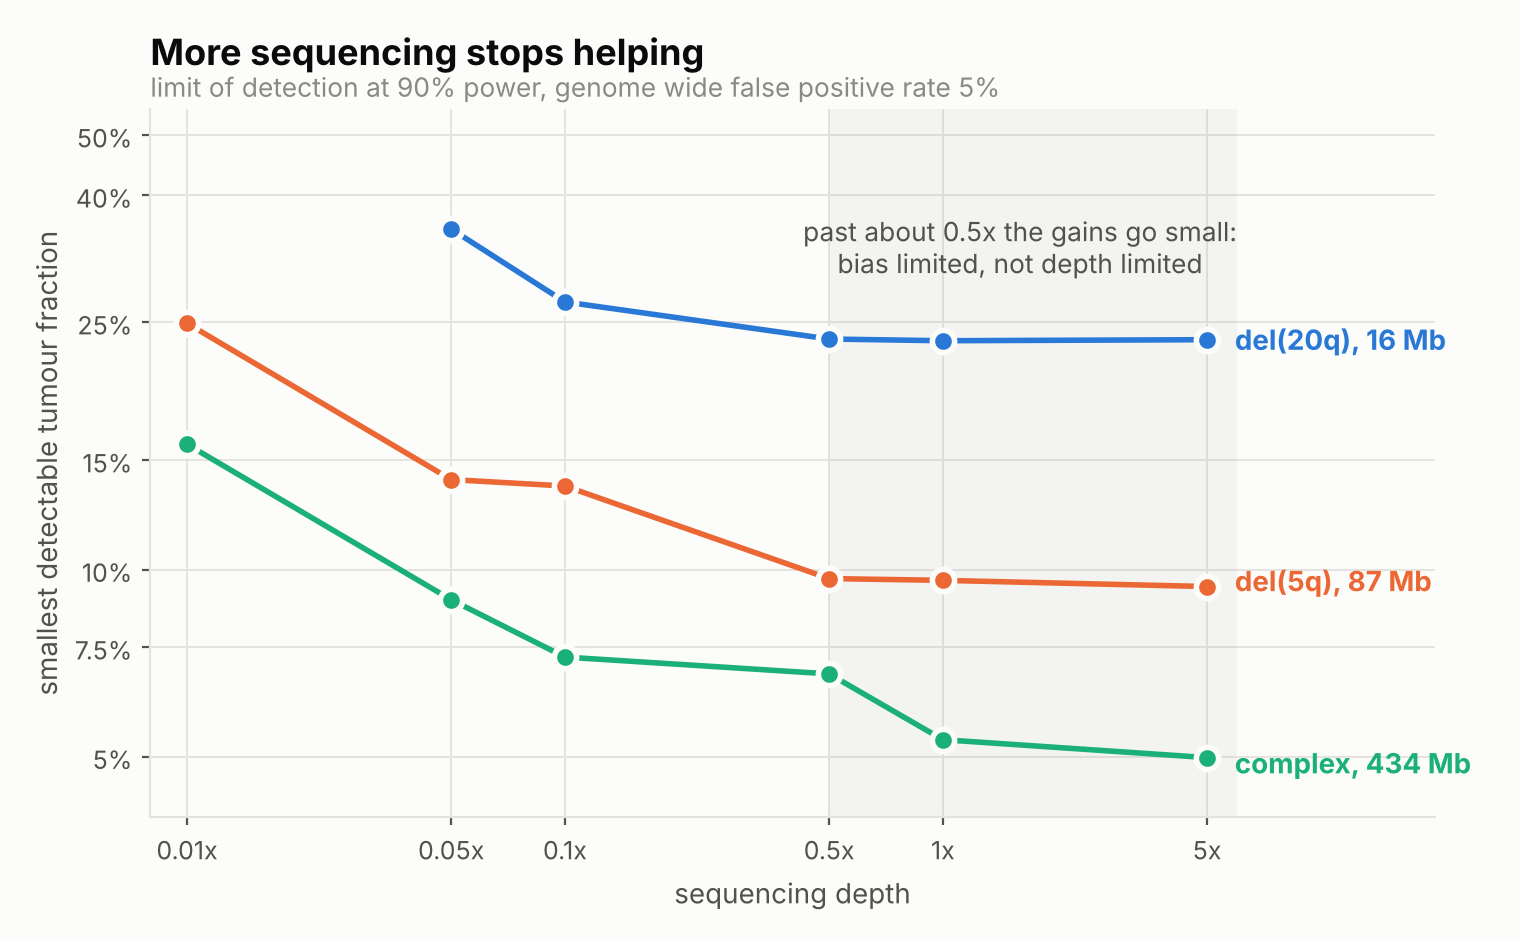
\includegraphics[width=\columnwidth]{fig1_depth_plateau.png}
\caption{Limit of detection against sequencing depth at 90 percent power and a
five percent genome-wide false positive rate. The curves flatten beyond
approximately 0.5$\times$, where library-to-library bias rather than counting
noise becomes the limiting factor.}
\label{fig:plateau}
\end{figure}

Table~\ref{tab:lod} gives the full surface. Increasing depth from 0.01$\times$
to 0.1$\times$ improves the detection limit by 45 to 58 percent, median 55.
Increasing it from 0.5$\times$ to 5$\times$, a tenfold increase in sequencing
cost, improves it by 0.3 to 27 percent, median 4.9, with six of eight lesions
gaining under nine percent. The single large gain belongs to the complex
karyotype, the easiest case, where the remaining headroom is comparable to the
resolution of the tumour-fraction grid.

\begin{table}[t]
\caption{Smallest tumour fraction detected with 90 percent probability.
``n.r.'' denotes not reached at any tumour fraction up to 40 percent.}
\label{tab:lod}
\centering
\begin{tabular}{lrrrrrr}
\toprule
Lesion & 0.01$\times$ & 0.05$\times$ & 0.1$\times$ & 0.5$\times$ & 1$\times$ & 5$\times$ \\
\midrule
del(20q), 5.5\,Mb  & n.r.  & n.r.  & 39.5 & 37.8 & 37.2 & 37.0 \\
del(20q), 16\,Mb   & n.r.  & 35.3 & 27.0 & 23.5 & 23.3 & 23.4 \\
del(13q), 33.5\,Mb & 38.3 & 23.0 & 21.1 & 14.3 & 13.9 & 13.9 \\
del(7q), 54\,Mb    & 35.9 & 22.1 & 16.3 & 13.7 & 13.4 & 12.8 \\
del(5q), 86\,Mb    & 24.9 & 14.0 & 13.6 & 9.7  & 9.6  & 9.4  \\
$+8$, 145\,Mb      & 23.7 & 13.1 & 10.0 & 8.1  & 7.3  & 7.4  \\
$-7$, 159\,Mb      & 23.2 & 13.2 & 10.5 & 9.2  & 9.0  & 8.1  \\
complex, 434\,Mb   & 15.9 & 8.9  & 7.2  & 6.8  & 5.3  & 5.0  \\
\bottomrule
\end{tabular}
\end{table}

The mechanism is visible in \eqref{eq:coverage}. At 0.01$\times$ the per-bin
Poisson variance dominates and additional reads reduce it directly. By
0.5$\times$ the counting noise has fallen below the variance contributed by
$u_i$, which does not shrink with depth at all. The practical implication is
blunt: a laboratory running 1$\times$ or 5$\times$ cell-free DNA for
cytogenetic purposes is purchasing coverage it cannot use, and the route past
the plateau is a better reference panel or a different class of evidence rather
than more reads.

\subsection{Detection scales with the square root of lesion size}

\begin{figure}[t]
\centering
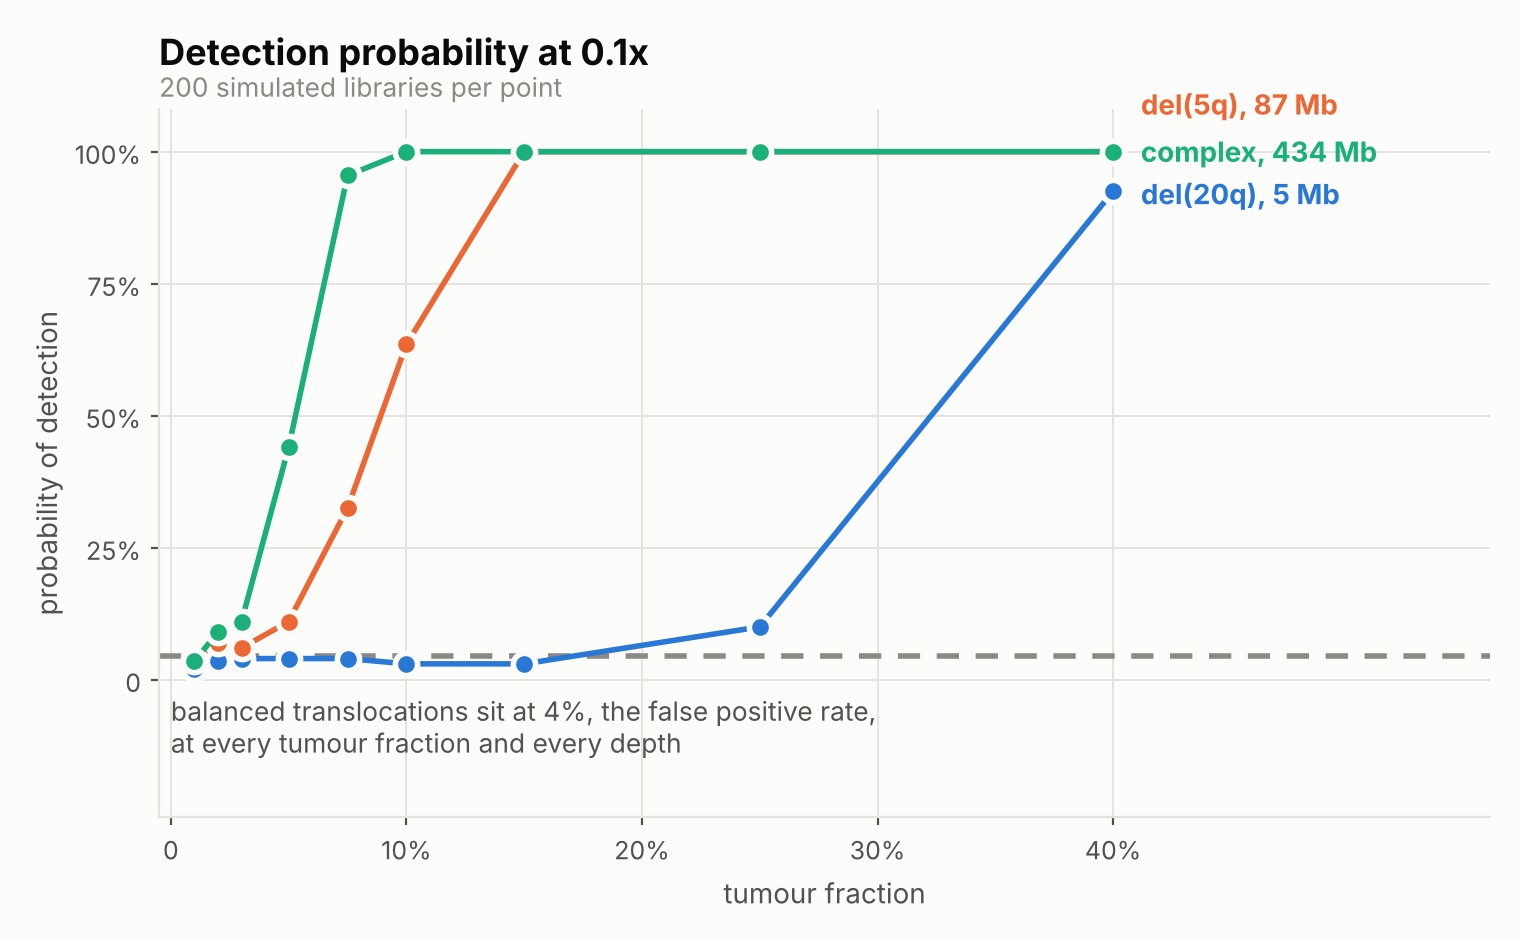
\includegraphics[width=\columnwidth]{fig2_power_curves.png}
\caption{Detection probability against tumour fraction at 0.1$\times$, with 200
simulated libraries per point. The dashed line is the false positive rate,
where every balanced rearrangement sits regardless of tumour fraction.}
\label{fig:power}
\end{figure}

Fitting the detection limit against lesion size on logarithmic axes gives a
slope of $-0.40$ at 0.1$\times$ and $-0.46$ at 5$\times$, close to the $-0.5$
implied by \eqref{eq:stouffer}: the segment statistic grows as the square root
of the number of bins averaged. Halving the detectable tumour fraction
therefore requires a lesion four times larger. This is not a tuning deficiency
but a property of averaging.

Localisation is not the limiting step. Among conditions at 0.1$\times$ reaching
90 percent detection, calls covered at least half the true lesion in 94 percent
of replicates. When the detector fires it fires in the right place; it does not
fire often enough.

\subsection{Balanced rearrangements are called at chance}

Across all 108 copy-neutral conditions, four rearrangements by six depths by
nine tumour fractions, mean detection was 5.3 percent against a five percent
false positive rate, with a maximum of 11.5 percent and a regression slope on
tumour fraction of $-0.007$, indistinguishable from zero.

This is the expected result and its absence would indicate a defect. The
simulator confirms the premise directly: a balanced rearrangement at 90 percent
tumour fraction yields a library numerically identical to a normal one under
the same random seed.

\subsection{The cost of junction-level evidence}

\begin{figure}[t]
\centering
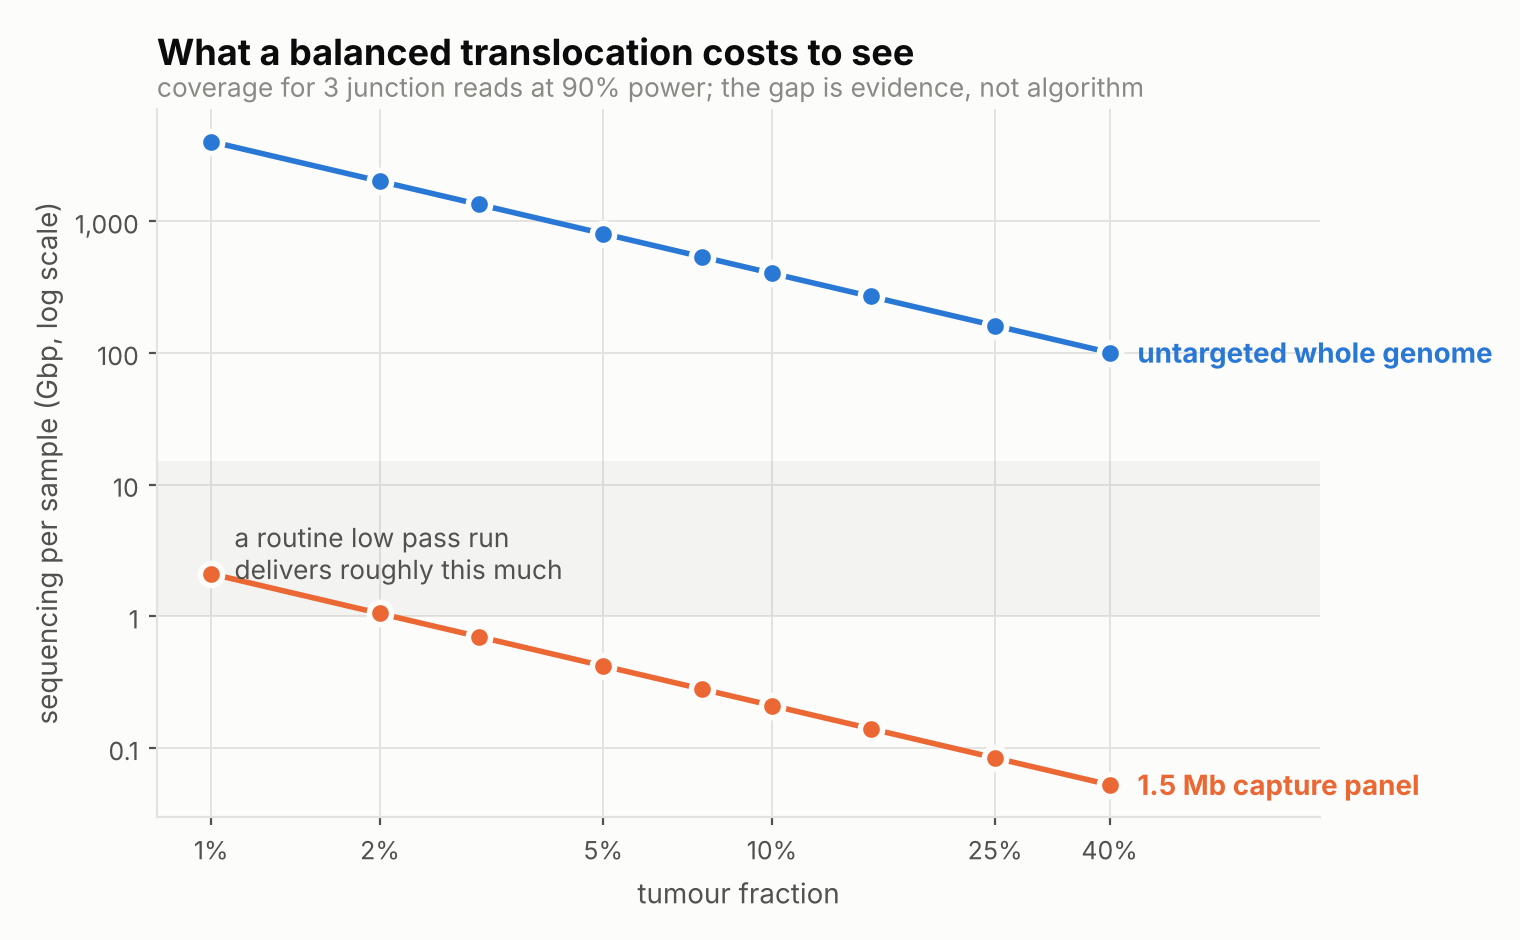
\includegraphics[width=\columnwidth]{fig3_junction_cost.png}
\caption{Sequencing required for three junction-spanning reads at 90 percent
power, untargeted against a 1.5\,Mb capture panel. The shaded band marks the
yield of a routine low-pass run.}
\label{fig:junction}
\end{figure}

By \eqref{eq:junction}, at 0.1$\times$ and ten percent tumour fraction the
expected usable junction evidence is 0.004 reads. This is not a detection
probability of 0.004; it is four thousandths of a single read.
Table~\ref{tab:junction} gives the coverage required for 90 percent power.

\begin{table}[t]
\caption{Sequencing required for three junction reads at 90 percent power.}
\label{tab:junction}
\centering
\begin{tabular}{lrrr}
\toprule
Tumour fraction & Coverage & Untargeted (Gbp) & Capture (Gbp) \\
\midrule
1\%  & 1400$\times$ & 4339 & 2.10 \\
2\%  & 700$\times$  & 2170 & 1.05 \\
5\%  & 280$\times$  & 868  & 0.42 \\
10\% & 140$\times$  & 434  & 0.21 \\
25\% & 56$\times$   & 174  & 0.08 \\
50\% & 28$\times$   & 87   & 0.04 \\
\bottomrule
\end{tabular}
\end{table}

A routine low-pass run delivers between one and 15\,Gbp. Untargeted sequencing
is short by two to three orders of magnitude. The recurrent haematological
fusion breakpoints occupy approximately 1.5\,Mb in total, 0.05 percent of the
genome, so a capture panel tiling them concentrates coverage by a factor of
about 2{,}000 and brings the same evidence within a fraction of a gigabase.

\section{Discussion}

The three findings have a common shape: each identifies a limit that is
structural rather than algorithmic, and each therefore redirects effort rather
than merely characterising it.

The plateau says that the marginal value of sequencing depth in this
application collapses early. Any effort spent on deeper low-pass sequencing is
better spent on reference-panel quality, since the panel is what removes the
bias component that depth cannot touch.

The size scaling says that sub-arm lesions are outside the reach of untargeted
low-pass sequencing at clinically interesting tumour fractions, and that no
reasonable improvement in calling changes this, because the exponent follows
from averaging rather than from implementation.

The junction calculation is the most consequential of the three, because it
closes a line of enquiry. Detecting balanced rearrangements from untargeted
low-pass cell-free DNA is not difficult, it is impossible at these budgets, and
the impossibility is arithmetic rather than methodological. Fragmentomic
approaches \cite{cristiano2019fragmentation} remain interesting for detecting
that an abnormal clone is present, but they cannot identify which rearrangement
it carries, because that information is carried only by molecules that cross
the junction.

What remains open is correspondingly narrower and more tractable. The design of
a minimal capture panel covering the recurrent fusions is a pure optimisation
problem on published breakpoint coordinates requiring no new data. Lowering the
supporting-read threshold defensibly would reduce the required coverage
proportionally. And the question of whether aggregate fragmentomic signal can
flag clonal presence without localisation is untouched by anything here.

\subsection{Limitations}

The per-library bias standard deviation is a reasoned estimate rather than a
fitted quantity, and it determines where the plateau sits. The existence of a
plateau follows from any non-zero value, but the specific depth should be read
as an order of magnitude. Fitting this parameter to real low-pass libraries is
the single highest-value extension of this work.

Our detector is of the correct class but is not WisecondorX or ichorCNA, and a
comparison against those implementations on the same simulated libraries is the
obvious next step. The direction of any discrepancy is not obvious: a
reimplementation may be weaker than a mature tool, but the genome-wide
calibration used here is stricter on specificity than some published pipelines.
The copy-neutral result is unaffected either way, since it depends on no
implementation detail.

GC content and mappability are modelled rather than measured, lesions are clean
where real karyotypes are subclonal and sometimes chromothriptic, and nothing
here has been validated against a sample of known karyotype and measured tumour
fraction. The study bounds what is possible under a stated model; it is not
evidence about any particular assay. A complete limitations register is
distributed with the code.

\section{Conclusion}

We measured, rather than assumed, what a bin-count copy-number caller can
detect in low-pass cell-free DNA across the lesion sizes that matter in
haematological malignancy. Sensitivity plateaus near 0.5$\times$ because
library-to-library bias rather than counting noise sets the floor; detection
scales with the inverse square root of lesion size, placing sub-arm lesions
outside reach at clinically relevant tumour fractions; and balanced
rearrangements are detected at exactly the false positive rate, with
junction-level evidence requiring coverage three orders of magnitude beyond a
low-pass run unless that coverage is concentrated by capture. The copy-neutral
blind spot is a problem of where the sequencing is pointed, not of how the
reads are analysed.

\section*{Reproducibility}

All code, simulated results, figures and the source of this manuscript are
available at \url{https://github.com/shubhodeepcx/low-pass-cfDNA} under an MIT
licence. The complete study runs in approximately five minutes on a laptop with
no reference genome or alignment files required.

\bibliographystyle{IEEEtran}
\bibliography{refs}

\end{document}
